\subsection{Cloud Service}\label{subsec:cloud-service}

\subsubsection{Architektur}

Der Cloud Service wird in die zwei Domänen Notification und Configuration aufgeteilt.
Dabei ist die Domäne Notification für das Versenden von Benachrichtigungen
und die Domäne Configuration für die Verwaltung und Auswertung der Konfigurationen verantwortlich.
Zwischen den beiden Domänen besteht eine gerichtete Abhängigkeit.
Die Domäne Notification benötigt zum Versenden von Benachrichtigungen Informationen aus der Configuration Domäne.
Das Identifizieren der relevanten Empfänger geschieht in der Configuration Domäne.
Dementsprechend benötigt die Notification Domäne beim Versenden die Information, an welche Empfänger die Benachrichtigung versendet werden soll.

Durch die klare Trennung der Verantwortungsbereiche der beiden Domänen, wäre es möglich diese in einzelne Microservices aufzuteilen.
Dies würde das Skalieren der Applikationen vereinfachen.
Die Aufteilung auf mehrere Microservices macht das System als ganzes aber komplexer.
Insbesondere Betrieb und Entwicklung wird aufwändiger, da diese Aufwände nun für mehrere Applikationen anfallen.
Für den Umfang dieser Arbeit wird deshalb darauf verzichtet, den Cloud Service als echtes Micro Service System umzusetzen.
Der Cloud Service wird als eine einzelne Spring Boot Applikation umgesetzt.
Innerhalb dieser Applikation sollen die Domänen Configuration und Notification allerdings, wo immer mit vertretbarem Aufwand möglich, getrennt bleiben.
Direkte Abhängigkeiten zwischen den beiden Domänen sind zu vermeiden.
An den Stellen wo Informationen aus der anderen Domäne nötig sind, sollen diese über ein Rest Interface abgefragt werden.
So kann die Applikation in Zukunft einfach und auf die tatsächlichen Bedürfnisse zugeschnitten in mehrere Microservices aufgeteilt werden.

Um einfache Erweiterbarkeit zu gewährleisten, wird der Cloud Service nach dem Prinzip von Onion Architecture aufgebaut.

\begin{figure}[h]
    \centering
    \begin{minipage}[b]{0.5\textwidth}
        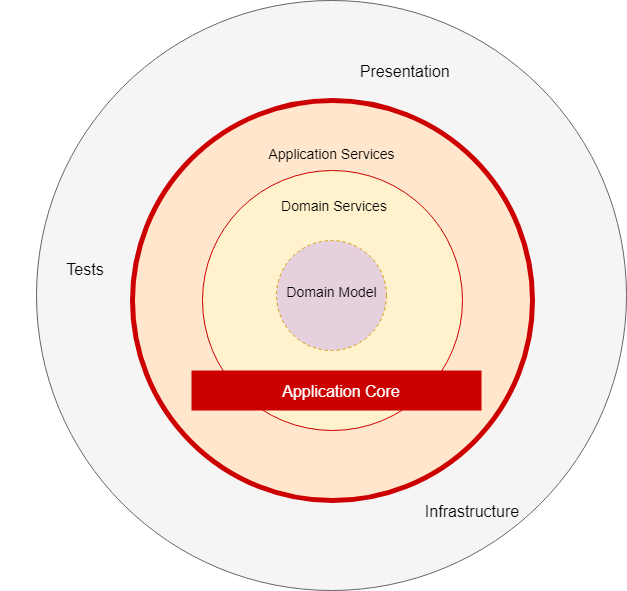
\includegraphics[width=\textwidth]{graphics/thinktocode-onion}
        \caption{Onion Architecture}
    \end{minipage}
\end{figure}

In Onion Architecture wird die Applikation in Layer aufgeteilt.\cite{medium-onion}
Im Zentrum des Modells steht die Domäne selbst.
Sie wird durch den Domain Layer abgebildet.
Der Domain Layer darf nur Abhängigkeiten auf sich selbst haben.
Umgekehrt dürfen aber alle anderen Layers Abhängigkeiten auf den Domain Layer haben.
Die nächste Schicht im Modell ist der Domain Service Layer.
Dieser bietet die fachliche Logik und definiert die Verhaltensweise des Domain Layers.
Der Layer Application Services bildet die Brücke zwischen externer Infrastruktur und Domain Services.
Dies beinhaltet Repository Services für die Schnittstelle zu persistentem Speicher und Rest Controllers für Schnittstellen zu anderen Applikationen.
In der äussersten Schicht steht der Infrastructure Layer.
Dieser beinhaltet externe Systeme, welche von der Applikation benötigt werden, wie Datenbanken, Messaging Services und Applikationen die auf Web APIs welche der Applikation zugreifen.

Um zu garantieren, dass keine ungewollten Abhängigkeiten zwischen Layern bestehen, können die Layers in eigene Module verpackt werden.
Dies erhöht jedoch die interne Komplexität der Applikation.
Das Onion Modell wird innerhalb des Cloud Services deshalb nicht durch Module, sondern durch eine vorgegebene Packagestruktur umgesetzt.

\begin{figure}[h]
    \centering
    \begin{minipage}[b]{0.9\textwidth}

        \dirtree{%
            .1 ch.fhnw.ip5.praxiscloudservice.
            .2 api.
            .2 config.
            .2 Domäne.
            .2 persistence.
            .2 service.
            .2 web.
        }
        \caption{Package Struktur Cloud Service}\label{fig:packagescloudservice}
    \end{minipage}
\end{figure}

Im Zentrum steht das Package Domäne.
Es beinhaltet alle Domänenobjekte und stellt alleine den Domäne Layer dar.
Der Domain Service Layer wird durch das Package Service abgebildet.
Hier werden sämtliche Domain Services implementiert.
Die Packages persistence und web beinhalten schliesslich den Application Service Layer.
Dabei definiert das Package persistence Services welche für Interaktion mit der Datenbank verwendet werden.
Das Package web definiert die REST-Endpunkte und Clients, welche für die Kommunikation zwischen den Domänen und anderen Services benötigt werden.
Die Objekte, welche darüber ausgetauscht werden, sind im Package api definiert.
So werden direkte Abhängigkeiten zwischen den Domänen Notification und Configuration vermieden.
Das Package api beinhaltet zudem Interfaces für Domain Services und Exceptions.
Diese werden im Package services implementiert und im package Web verwendet.
Letztlich beinhaltet das config die technische Konfiguration der Applikation.

\clearpage

\subsubsection{Domäne Configuration}

\begin{figure}[h]
    \centering
    \begin{minipage}[b]{0.9\textwidth}
        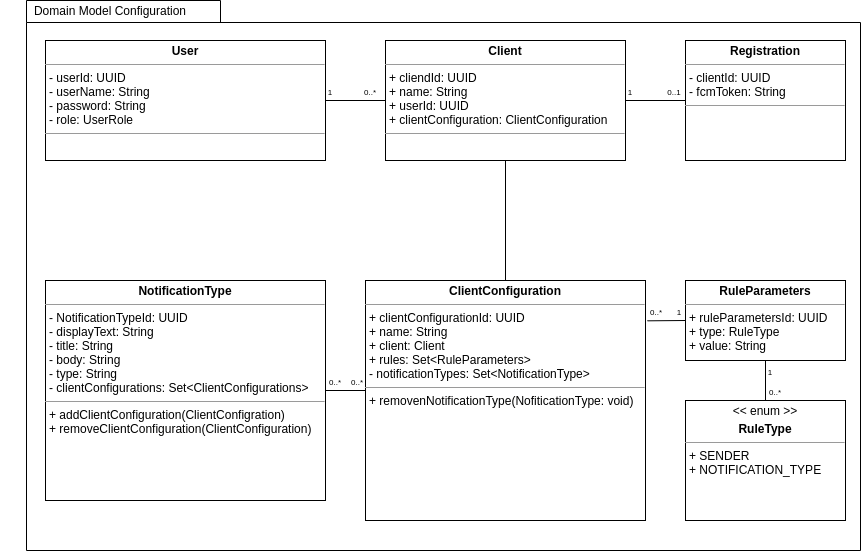
\includegraphics[width=\textwidth]{graphics/Class_Configuration_Domain}
        \caption{Domänenmodell Configuration}
    \end{minipage}
\end{figure}

Das Herzstück der Configuration Domäne ist die ClientConfiguration.
Die ClientConiguration beinhaltet die Informationen, welche Benachrichtigung ein Endgerät versenden kann und welche Benachrichtigungen es empfangen soll.
Ein Endgerät wird dabei durch die Entität Client dargestellt.
Client und ClientConfiguration sind getrennt, damit Clients auch ohne Configuration erfasst werden können.
So kann ein Administrator bereits Geräte im System erfassen, ohne Sie vollständig zu konfigurieren.
Die konkrete Konfiguration von Benachrichtigungen erfolgt über die Entitäten NotificationType und RuleParameters.
Ein NotificationType ist die Grundlage für eine Benachrichtigung.
Er definiert den Inhalt, der mit einer Benachrichtigung versendet wird.
Die Liste von NotificationTypes auf einer ClientConfiguration definiert, welche Benachrichtigungen der zugehörige Client versenden kann.
Welche Benachrichtigungen ein Client empfängt, wird über die Liste von RuleParameters auf der ClientConfiguration definiert.
Die konfigurierten RuleParameters werden von der RulesEngine ausgewertet, um relevante Empfänger für eine Benachrichtigung zu finden.
Dabei kann die Entität RuleParameters für alle Regeln wiederverwendet werden.
Die RuleEngine kann anhand des RuleType bestimmen, wie RuleParameters ausgewertet werden.

Zur Verwaltung von Konfigurationen wird weiter die Entität PraxisUser definiert.
Sie stellt einen Benutzer des Praxisrufsystems dar.
Jeder Benutzer kann die Rollen Admin oder User haben.
Ein Benutzer mit der Rolle Admin hat Recht die Konfiguration über das Admin UI zu verwalten.
Ein Benutzer mit der Rolle User ist berechtigt, den Mobile Client zu verwenden.

Für die Anbindung an den Messaging Service ist zudem die Entität Registration notwendig.
Die Registrierung eines Clients beinhaltet die technische Identifikation, mit der ein Client sich beim Messaging Service registriert hat.
Ein Client kann immer nur genau eine Registration haben.

\clearpage

\begin{figure}[h]
    \centering
    \begin{minipage}[b]{0.9\textwidth}
        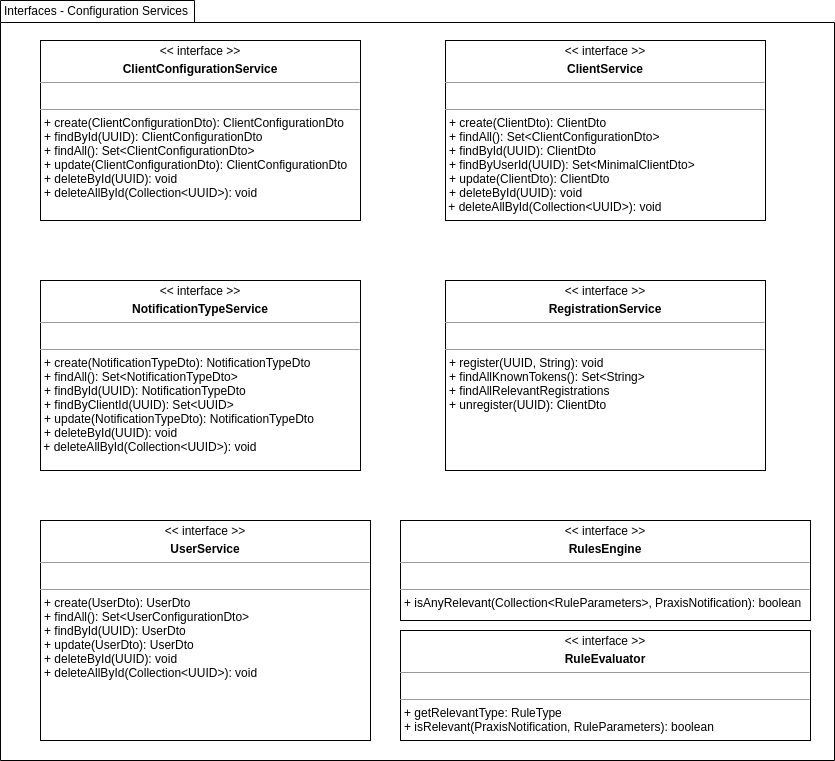
\includegraphics[width=\textwidth]{graphics/Class_Configuration_Services}
        \caption{Klassendiagramm Configuration Service Interfaces}
    \end{minipage}
\end{figure}

Die Configuration Domäne beinhaltet Services zum Lesen, Erstellen, Ändern und Löschen der Domänenobjekte.
Diese Verwaltungsfunktionen werden über eine REST-API exponiert. \footnote{Siehe Kapitel 5.3.4}
Der RegistrationService bietet dabei eine Ausnahme.
Er bietet die Funktionen, Registrierungen zu erfassen und aktualisieren.
Diese werden verwendet, wenn sich ein Mobile Client beim Cloud Service registriert.
Er bietet zudem die Möglichkeit die Identifikation (Token) aller relevanten Empfänger für eine gegebene Benachrichtigung zu finden.
Diese Auswertungen werden mithilfe der RulesEngine gemacht.
Die RulesEngine bewertet die erfassten RulesParameter mithilfe der RuleEvaluators und findet alle relevanten Einträge.

Die RulesEngine ermöglicht es, dem Cloud Service festzustellen, welche Benachrichtigungen an welche Clients versendet werden sollen.
Dazu bietet sie eine einzelne öffentliche Methode.
Diese nimmt eine Liste von Regelparametern (RulesParameters) und eine Notification entgegen.
Zurückgegeben wird ein Boolean Wert, der sagt, ob mindestens eine der übergebenen Regelparameter für die Benachrichtigung relevant ist.
Da jeder aktive Client eine ClientConfiguration definiert, die eine Liste an Regelparametern beinhaltet kann so mit der RulesEngine bewertet werden, ob ein bestimmter Client sich für eine Benachrichtigung interessiert.

\begin{figure}[h]
    \centering
    \begin{minipage}[b]{0.9\textwidth}
        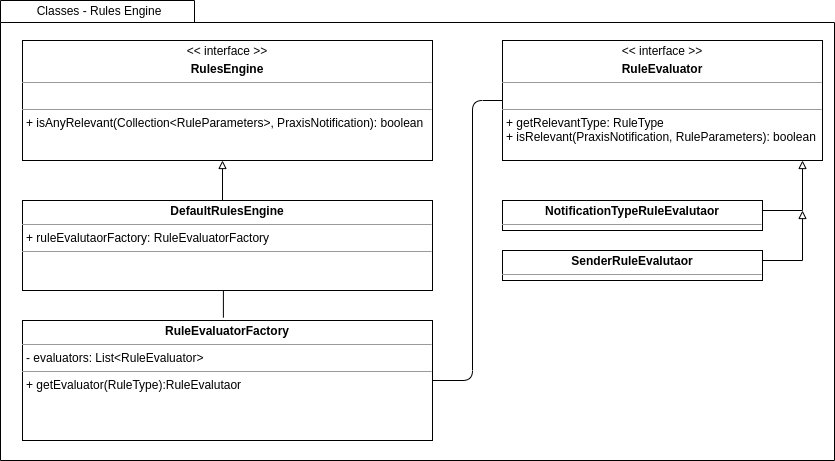
\includegraphics[width=\textwidth]{graphics/Class_Configuration_RulesEngine}
        \caption{Klassendiagramm Rules Engine}
    \end{minipage}
\end{figure}

Die Auswertung der einzelnen Regelparameter innerhalb der RulesEngine wird an einzelne RuleEvaluatoren delegiert.
Umgesetzt wird dieses Konzept mit einem Strategy Pattern.\cite{design-patterns}
RuleEvaluator definiert das Strategy Interface.
Der Zugriff auf die einzelnen Strategies innerhalb der RulesEngine wird über eine RuleEvaluatorFactory gelöst.
Diese Factory kennt alle existierenden RuleEvaluator Instanzen und bietet eine öffentliche Methode, über welche der RuleEvaluator für einen bestimmten Typ geladen werden kann.
Über die Dependency Injection des Spring Frameworks, kann diese RuleEvaluatorFactory einfach und erweiterbar implementiert werden:

\lstinputlisting[caption=RuleEvaluatorFactory.java,language=java,label={lst:RuleEvaluatorFactory.java}]{listings/RuleEvaluatorFactory.java}

Über den @Autowired Konstruktor nimmt die Factory eine Liste des Types RuleEvaluator entgegen.
Die Spring Dependency Injection wird hier automatisch alle verfügbaren RuleEvaluator Instanzen in einer Liste sammeln und als Konstruktorparameter entgegennehmen.
Da jeder RuleEvaluator eine Methode bietet, über die der relevante RuleType abgefragt werden kann, kann nun aus dieser Liste eine Map gebaut werden, die RuleTypes auf die relevanten RuleEvaluator Instanzen mapped.
Das Laden eines RuleEvaluators anhand des RuleTypes kann nun über ein einfaches Lookup in der Map erfolgen.
Werden in der Zukunft weitere RuleTypes unterstützt, reicht es den entsprechenden RuleEvaluator zu implementieren.
Der neue RuleEvaluator wird danach automatisch über die RuleEvaluatorFactory verfügbar sein.
Anpassungen an der RulesEngine oder der RuleEvaluatorFactory sind nicht nötig.

\clearpage

\subsubsection{Domäne Notification}

\begin{figure}[h]
    \centering
    \begin{minipage}[b]{1.0\textwidth}
        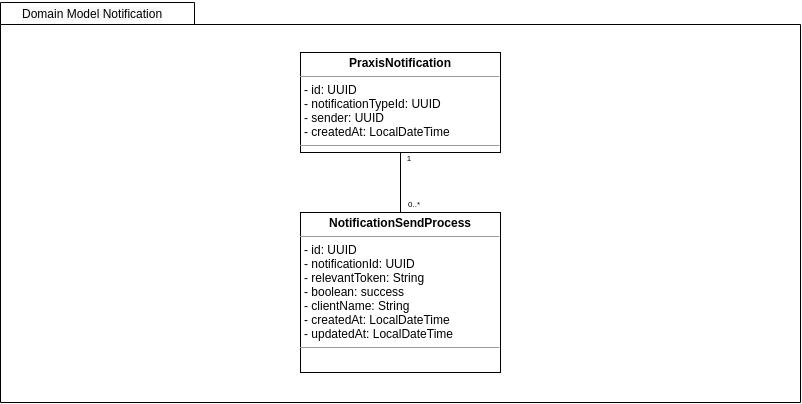
\includegraphics[width=\textwidth]{graphics/Class_Notification_Domain}
        \caption{Domänenmodell Notification}
    \end{minipage}
\end{figure}

In der Domäne Notification werden zwei Entitäten definiert.
Die Entität PraxisNotification stellt eine Benachrichtigung dar, die über den Cloud Service versendet wird.
Jede Notification die der CloudService erhält wird bereits vor dem Versenden persistiert.
Nach dem eine Benachrichtigung als PraxisNotification persistiert wurde, wird sie an die Empfänger versendet.
Dabei wird für jeden Empfänger ein SendNotificationProcess erstellt.
Dieser SendNotificationProcess beinhaltet eine Referenz auf die versendete Benachrichtigung und den Status des Sendeprozesses.
Dies dient zum einen der Nachvollziehbarkeit.
Zum anderen ermöglicht es, fehlgeschlagene Benachrichtigungen nur für die Empfänger zu wiederholen, für die der Versand fehlgeschlagen ist.

\begin{figure}[h]
    \centering
    \begin{minipage}[b]{0.9\textwidth}
        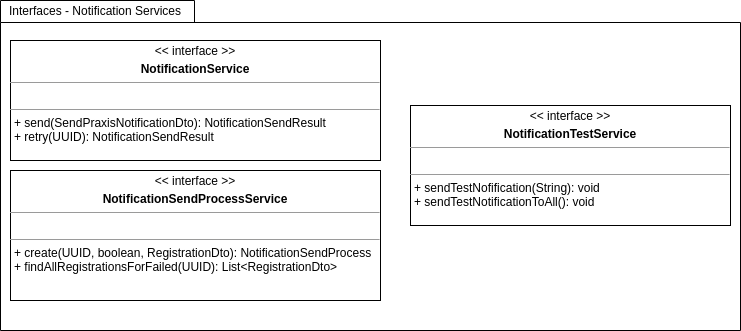
\includegraphics[width=\textwidth]{graphics/Class_Notification_Services}
        \caption{Klassendiagramm Notification Service Interfaces}
    \end{minipage}
\end{figure}

In der Notification Domäne werden drei Domain Services definiert.
Der NotificationService bietet Methoden, um eine Notifikation zu versenden und zu wiederholen.
Für das initiale Versenden werden die Informationen benötigt, um eine Notifikation zu erstellen und die Empfänger zu identifizieren.
Im Fall der Wiederholung werden diese Informationen nicht mehr benötigt.
Die Notifikation und der Status des Versandprozesses wurden beim ersten Versuch sie zu versenden bereits persistiert.
Als zweiter Service definiert der NotificationSendProcessService dazu Sendevorgänge zu erstellen und fehlgeschlagene Sendevorgänge zu finden.
Der dritte Service in der Notification Domäne dient nur zu Test- und Administrationszwecken.
Der NotificationTestService kann verwendet werden, um einem einzelnen Client eine Testnachricht zu senden oder allen registrierten Clients eine Nachricht zu schicken.
Als Benachrichtigung wird dabei immer eine vom Cloud Service definierte Benachrichtigung versendet, welche nur Platzhalterwerte beinhaltet.

\subsubsection{Laufzeitmodell}

Im Folgenden werden die Abläufe für die Registrierung von Mobile Clients sowie das Versenden und Empfangen von Benachrichtigungen im Detail definiert.

\subsubsection*{Client Registration}

Damit ein Client Benachrichtigungen empfangen und versenden kann, muss er sich bei Messaging Service und Cloud Service registrieren.
Hier wird dieser Ablauf spezifiziert.
Als Vorbedingung wird dabei angenommen, dass mindestens ein Client inklusive ClientConfiguration erfasst und dem Praxismitarbeitenden zugewiesen wurde.

\begin{figure}[h]
    \centering
    \begin{minipage}[b]{0.7\textwidth}
        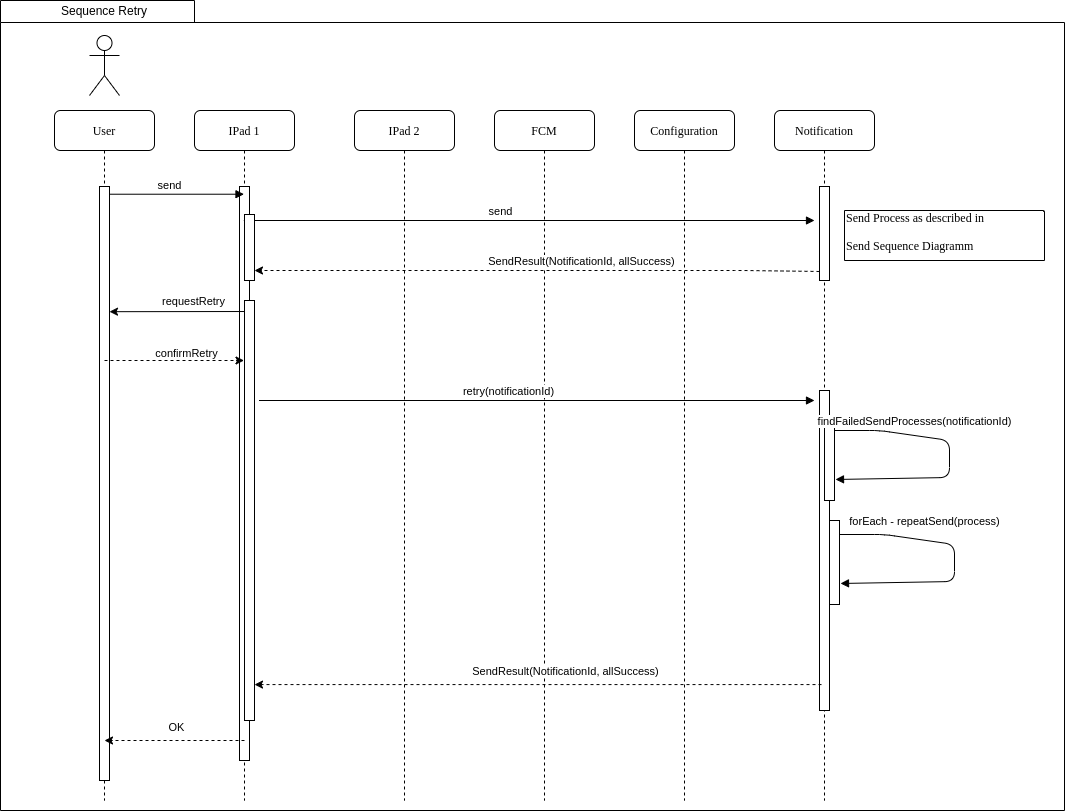
\includegraphics[width=\textwidth]{graphics/Sequence_Notification_Register}
        \caption{Ablauf Registration}
    \end{minipage}
\end{figure}

In einem ersten Schritt muss sich der Praxismitarbeiter im Mobile Client anmelden.
Die Anmeldung wird im Cloud Service ausgewertet.
Hat er gültige Benutzerdaten angegeben, werden Informationen zu allen verfügbaren Konfigurationen vom Cloud Service geladen und der Benutzer kann die gewünschte Konfiguration auswählen.
Dabei werden nur Name und Id der Konfigurationen geladen, damit nicht mehr Daten als nötig übertragen werden.
Wählt Benutzer die gewünschte Konfiguration, werden alle dafür konfigurierten NotificationTypes geladen und im UI die entsprechenden Buttons erstellt.
Direkt nach dem Laden der Konfiguration registriert sich der Mobile Client beim Messaging Service.
Als Antwort erhält er ein eindeutiges Token, welches verwendet werden kann, um an diesem Client Nachrichten zu senden.
Der Mobile Client registriert sich darauf mit dem erhaltenen Token und der ausgewählten Konfiguration beim Cloud Service.
Nach diesem Ablauf ist der Client bei Messaging Service und Cloud Service registriert und bereit Benachrichtigungen zu empfangen.

\subsubsection*{Benachrichtigung versenden und empfangen}

Die zentrale Funktion des Praxisrufsystems ist das Versenden und Empfangen von Benachrichtigungen.
Hier wird dieser Ablauf im Erfolgsfall beschrieben.
Als Vorbedingung wird angenommen, dass Konfiguration und Registrierung gemäss Abbildung 5.14 für zwei Clients abgeschlossen ist.
Dabei ist einer der Clients konfiguriert, Benachrichtigungen vom anderen Client zu empfangen.

\begin{figure}[h]
    \centering
    \begin{minipage}[b]{0.9\textwidth}
        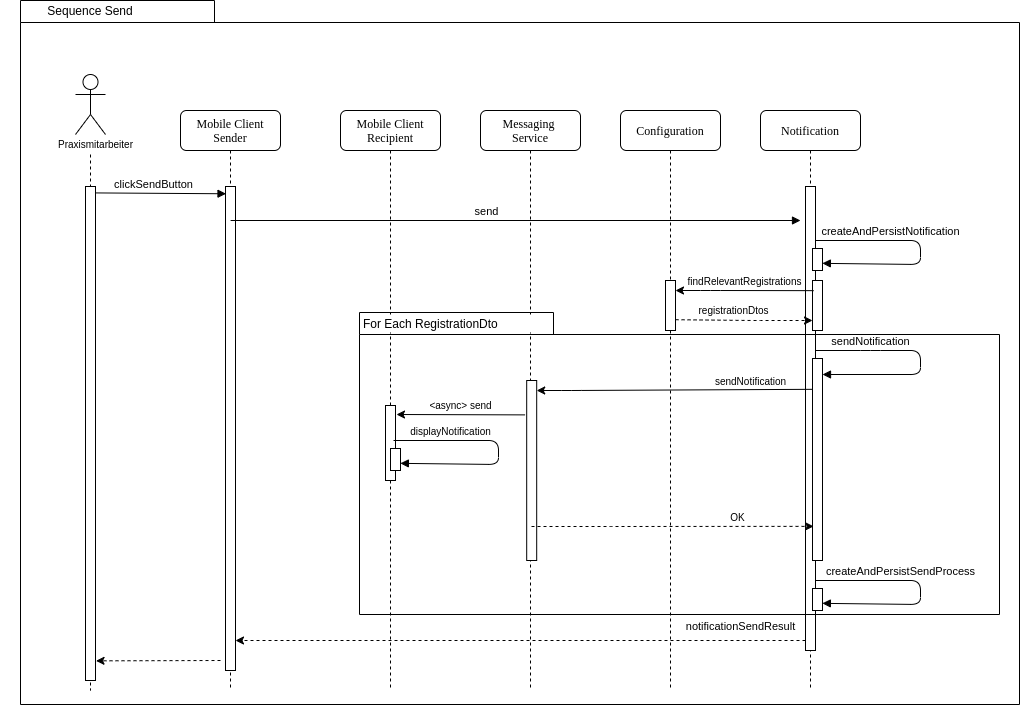
\includegraphics[width=\textwidth]{graphics/Sequence_Notification_Send}
        \caption{Ablauf Benachrichtigung Senden und Empfangen}
    \end{minipage}
\end{figure}

Nachdem der Benutzer das Versenden einer Benachrichtigung auslöst, wird eine Anfrage an den NotificationController im Cloud Service gesendet.
Darin enthalten sind die Id des Senders sowie die Id des NotificationTypes.
Der NotificationController macht in der Folge eine Anfrage an den ConfigurationController, um alle relevanten Empfänger zu finden.
Im ConfigurationController werden die erfassten RuleParameters aller konfigurierten ClientConfigurations ausgewertet.
Darauf wird eine Liste der Registrierungen aller relevanten Empfänger zurückgegeben.
Sobald die Empfänger geladen sind, erstellt der NotificationController eine Benachrichtigung aus dem gegebenen NotificationType.
Diese Benachrichtigung wird als PraxisNotification persistiert und an den MessagingService übergeben.
Der Messaging Service stellt die Zustellung anhand der mitgegebenen Registrierung sicher.
Nach der Übermittlung an den Messaging Service wird im CloudService pro Empfänger ein NotificationSendProzess erstellt der den Status für diesen Empfänger dokumentiert.
Der NotificationController sendet darauf eine Bestätigung an den Mobile Client.
Diese Antwort beinhaltet die technische Id der versendeten Benachrichtigung und das Resultat, ob die Benachrichtigung an alle Empfänger versendet werden konnte.
Auf Empfängerseite wird die Benachrichtigung verarbeitet und angezeigt, sobald die Zustellung durch den Messaging Service erfolgt ist.
Diese Zustellung erfolgt asynchron.
Dementsprechend kann der Sender nur informiert werden, wenn die Zustellung an den Messaging Service fehlgeschlagen ist.

\clearpage
\subsubsection*{Benachrichtigung wiederholen}

Die zentrale Funktion des Praxisrufsystems ist das Versenden und Empfangen von Benachrichtigungen.
Hier wird dieser Ablauf im Fehlerfall beschrieben.
Als Vorbedingung wird angenommen, dass Konfiguration und Registrierung gemäss Abbildung 5.14 für zwei Clients abgeschlossen ist.
Dabei ist einer der Clients konfiguriert, Benachrichtigungen vom anderen Client zu empfangen.
Es wurde eine Benachrichtigung gemäss Abbildung 5.15 versendet, das Versenden an mindestens einen Client ist fehlgeschlagen
und der Cloud Service hat ein negatives SendNotificationResult zurückgegeben.

Nach dem Erhalt des negativen Resultats zeigt der Mobile Client einen Dialog an.
Dieser Dialog informiert den Benutzer über den Fehler und fragt an, ob die fehlgeschlagenen Benachrichtigungen wiederholt werden sollen.
Bestätigt der Benutzer wird diese Anfrage, wird eine Anfrage an den NotificationController gesendet um das Versenden zu wiederholen.
Diese Anfrage beinhaltet die technische Id der fehlgeschlagenen Benachrichtigung.
Der NotificationController findet alle negativen Einträge für diese Benachrichtigung in der NotificationSendProcess Tabelle.
Anschliessend wird jeder gefundene SendProcess anhand der Tokens in dieser NotificationSendProcess Instanzen wiederholt.
Das Versenden, Empfangen und die Rückmeldung an den Mobile Client erfolgen analog zum Ablauf "Benachrichtigung versenden und empfangen".

\begin{figure}[h]
    \centering
    \begin{minipage}[b]{0.9\textwidth}
        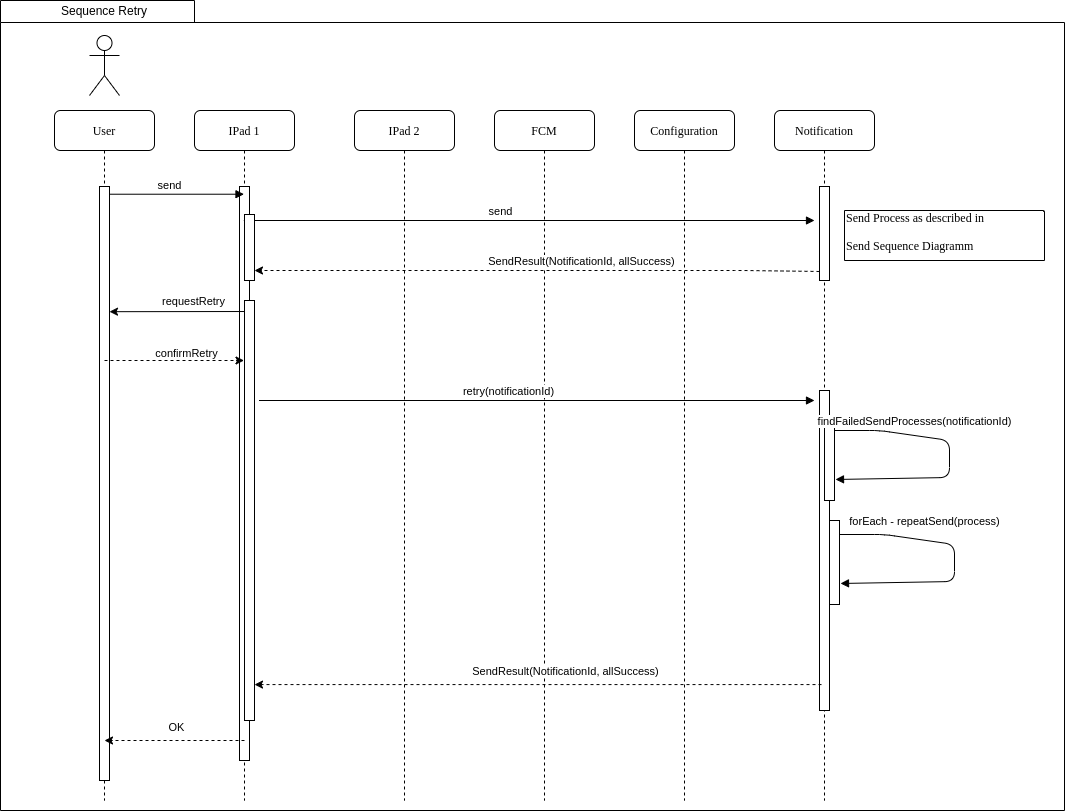
\includegraphics[width=\textwidth]{graphics/Sequence_Notification_Retry}
        \caption{Ablauf Benachrichtigung Wiederholen}
    \end{minipage}
\end{figure}


\clearpage

\subsubsection{API}

Um die Verwaltung der Konfigurationen zu ermöglichen, bietet der Cloud Service eine REST-API an.
Der Cloud Service bietet Verwaltungs-APIs für die folgenden Domänenobjekte:

\begin{tabularx}{\textwidth}{|l|X|}
    \hline
    \textbf{Domänenobjekt} & \textbf{Entity Name}  \\
    \hline
    Client                 & clients               \\
    \hline
    Client Configuration   & client-configurations \\
    \hline
    Notification Types     & notification-types    \\
    \hline
    Users                  & users                 \\
    \hline
\end{tabularx}\label{tab:adminapimethods}

Für jedes dieser Domänenobjekte ist ein dedizierter Endpunkt definiert, der unter dem Pfad /api/entity-name erreichbar ist.
Jeder dieser Kontroller bietet eine API zu Verwaltung dieses Domänenobjekts, welche dem folgenden Schema folgt:

\begin{tabularx}{\textwidth}{|p{5cm}|l|l|l|X|}
    \hline
    \textbf{Action}            & \textbf{HTTP} & \textbf{Pfad}        & \textbf{Body} & \textbf{Response} \\
    \hline
    Alle Elemente lesen        & GET           & /api/entity-name     & -             & [EntityDto]       \\
    \hline
    Einzelnes Element lesen    & GET           & /api/entity-name/id  & -             & EntityDto         \\
    \hline
    Neues Element erstellen    & POST          & /api/entity-name     & EntityDto     & EntityDto         \\
    \hline
    Bestehendes Element ändern & PUT           & /api/entity-name     & EntityDto     & EntityDto         \\
    \hline
    Einzelnes Element löschen  & DELETE        & /api/entity-name/id  & -             & -                 \\
    \hline
    Mehrere Elemente löschen   & DELETE        & /api/entity-name/ids & -             & -                 \\
    \hline
\end{tabularx}\label{tab:apimethods}

Eine Ausnahme, bildet hier das Domänenobjekt Registration.
Hier wird analog zum Domänenservice für Registrations\footnote{Siehe Kapitel 5.3.2} folgende API angeboten:

\begin{tabularx}{\textwidth}{|p{5cm}|l|l|X|X|}
    \hline
    \textbf{Aktion}                & \textbf{HTTP} & \textbf{Pfad}             & \textbf{Body}   & \textbf{Response} \\
    \hline
    Registrierung aktualisieren    & POST          & /api/registrations       & ClientId, Token & -                 \\
    \hline
    Registrierung entfernen        & DELETE        & /api/registrations       & ClientId        & -                 \\
    \hline
    Relevante Registrierung finden & POST          & /api/registrations/tokens & Notification-Dto & [Registration-Dto] \\
    \hline
\end{tabularx}\label{tab:registrationsapimethods}

\subsubsection*{Benachrichtigungen}

Zum Versenden von Benachrichtigungen bietet der Cloud Service folgende Endpunkte an:

\begin{tabularx}{\textwidth}{|p{5cm}|l|l|l|X|}
    \hline
    \textbf{Aktion}                  & \textbf{HTTP} & \textbf{Pfad}            & \textbf{Body}   & \textbf{Response}       \\
    \hline
    Nachricht versenden              & POST          & /api/notifications/send & NotificationDto & Notification-Response-Dto \\
    \hline
    Fehlgeschlagene erneut versenden & POST          & /api/notifications/retry & NotificationId  & Notification-Response-Dto \\
    \hline
\end{tabularx}\label{tab:registrationsapimethodss}

\clearpage

\subsubsection{Authentifizierung}
Die Authentifizierung von Benutzern wird mittels Spring-Security gelöst.
Der Einfachheit halber werden die User in einer eigenen Datenbanktabelle verwaltet.
Mit einem vertretbaren Mehraufwand könnte diese Verantwortlichkeit jedoch auch noch an einen externen Provider wie z.B. Keycloack delegiert werden.

Der User authentifiziert sich mit seinem Username und Passwort (BasicAuth) erstmalig über den Login-Endpoint.
Der Cloud Service stellt mit dem DefaultUserService eine eigene Implementation für die von Spring-Security verwendeten Komponenten UserDetailsService und AuthenticationProvider bereit (siehe Abbildung 5.18).
Hier werden die übergebenen Credentials überprüft und bei erfolgreicher Anmeldung ein Authentication Objekt mit den entsprechenden Benutzerrollen im Security-Context abgelegt.\cite{basicAuth}

Aus diesem Objekt wird ein JWT-Token generiert, welches 24h lang gültig ist und dem Client zurückgegeben.
Für alle weiteren Request während der laufenden Session authentifiziert sich der Client mit diesem JWT-Token (BarearToken Auth).

\begin{figure}[h]
    \centering
    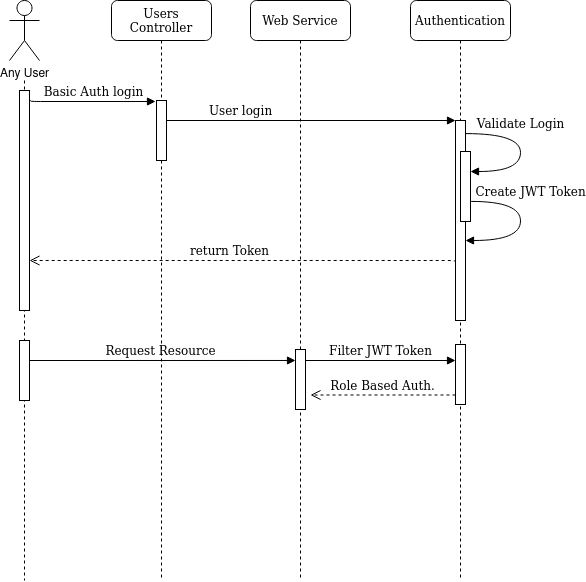
\includegraphics[width=0.5\textwidth]{graphics/Authentication-export}\caption[Authentifizierung-Sequenz]{Authentifizierung-Sequenz}
\end{figure}

Der Vorteil an JWT ist dabei, dass zum einen keine SessionId als Cookie im Browser gespeichert wird.\cite{tokenVsSessionId}
Und zum Anderen, dass innerhalb des JWT Tokens zusätzliche Metadaten gespeichert werden können.\cite{jwtIntro}
Wir verwenden dies um die Rolle sowie die Id des Benutzers bei den Requests mitliefern zu können.

\clearpage
\begin{figure}[h]
    \centering
    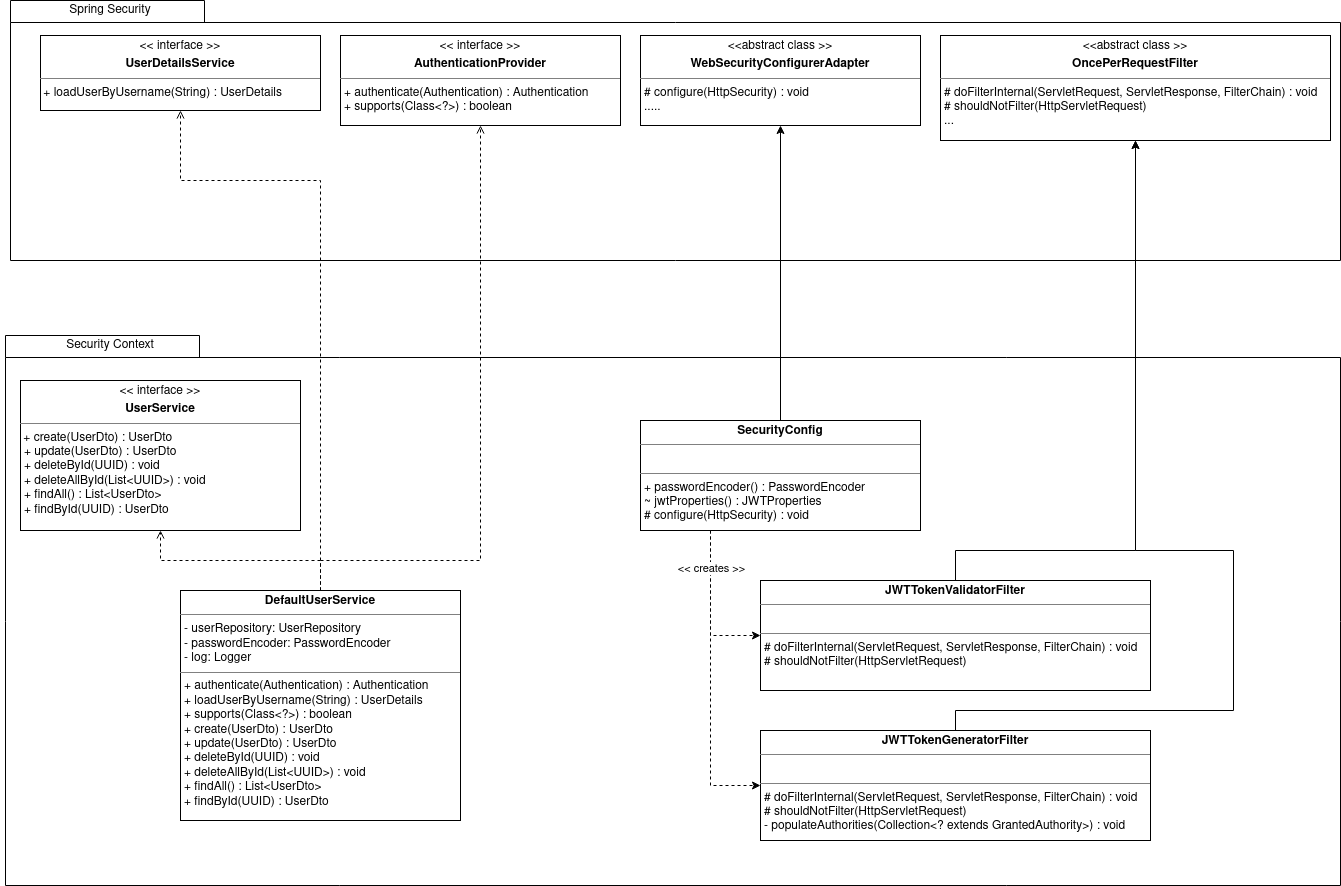
\includegraphics[width=0.9\textwidth]{graphics/SecuirtyContextClassDiagram-export}\caption[SecurityContext-Klassendiagram]{SecurityContext-Klassendiagram}
\end{figure}\label{fig:securityclassdiagram}

\subsubsection{Autorisierung}
Aktuell werden die Rollen User und Administrator verwendet.
Das Rollensystem lässt sich ohne grösseren Aufwand beliebig im entsprechenden Enum erweitern.
Die Abfrage der Berechtigung wird für das gesamte System zentral in der SecurityConfig (Siehe Abbildung 5.18) geprüft.
Dabei werden die entsprechenden Rollen für den jeweiligen HTTP-Request abgefragt.

\clearpage
